% !TeX encoding = UTF-8

\chapter{IMPLEMENTAÇÃO}\label{ch:implementacao}

Neste capítulo serão abordadas questões do planejamento e da implementação do sistema de reconhecimento de faces em vídeo. Primeiramente, os requisitos do sistemas serão analisados e descritos, seguidos da modelagem destes requisitos em forma de fluxograma, seguidos da modelagem das classes que serão criadas por meio dos diagramas descritos na \autoref{subsec:uml}, e por fim, as questõs de configuração do ambiente de desenvolvimento e a implementação efetiva do código. Todo este processo é feito seguindo conceitos da metodologia ágil XP, descrita na \autoref{subsec:devagil}.

\section{Análise de Requisitos}\label{sec:analiserec}
Para que se possa iniciar o planejamento da implementação do sistema aqui proposto por meio de diagramação, deve-se colher os requisitos necessários para o funcionamento do sistema. Ou seja, analisar o problema descrevendo entredas e saidas de dados, todas as situações e seus fluxos de informações. Sendo assim lista-se por ordem de execução os requisitos que atendem à proposta do sistema, discriminados por \textbf{entrada}, \textbf{processamento} e \textbf{saída} de dados ou informações:

\begin{enumerate}
	\item \textbf{entrada:} uma câmera do tipo \textit{webcam} descrita na \autoref{sec: tec-ferramenta} deve estar filmando uma área com iluminação controlada, produzindo o fluxo de \textit{frames} e disponibilizando em formado digital para o sistema;
	
	\item \textbf{processamento:} o sistema adquire controle do fluxo de \textit{frames} da \textit{webcam}, manipulando-o para que se possa ser exibido na tela do microcomputador e realiza a detecção de uma face, em tempo real, utilizando o algoritmo descrito na \autoref{subsubsec:violajones} com os materiais contemplados na \autoref{subsec:bib_opencv};
	
	\item \textbf{saída:} o sistema exibe, em tempo real, o fluxo de \textit{frames} processado como define o item acima, na tela do microcoputador. Ao mesmo tempo, caso seja detectada uma face, o sistema deverá desenhar um retângulo em volta da face detectada neste fluxo de \textit{frames}, ativando um campo para que o usuário possa entrar com uma identificação da face detectada;
	
	\item \textbf{entrada:} o usuário entra com uma identificação da face detectada, caso haja, em um campo disponibilidado pelo sistema (por exemplo, um nome);
	
	\item \textbf{processamento:} o sistema inicia o processo de treinamento da face definido na \autoref{sec:recog_faces}, criando um \textit{eigenspace}, e no momento seguinte à criação deste "plano cartesiado", o sistema já deve realizar o processo de reconhecimento descrito na \autoref{subsec:reconhecimento};
	
	\item \textbf{saída:} caso seja reconhecida uma face no fluxo de \textit{frames}, tal como descrito no item acima, o sistema deve exibir a identificação introduzida pelo usuário com define o item "4";
\end{enumerate}



\section{Diagrama de Fluxo de Dados}\label{sec:fluxorec}

O diagrama de fluxo é uma técnica que apresenta de forma gráfica, sequêncial, as atividades de um processo para facilitar a visualização de suas etapas \cite{fluxogramalivro}.

Na elaboração deste diagrama, considera-se que os requisitos listados na seção 4.1"ocorrem em tempo-real. Sendo assim, todas as tarefas necessárias para atender os requisitos devem ser executados em um \textit{loop}, exceto para o requisito de entrada identificação da face (item 4) e o requisito de treinamento (item 5, de processamento), que ocorrerão apenas caso o usuário introduza a informação.

A fluxograma da \autoref{fig:fluxoreq} dispõe os requisitos e o diagrama de fluxo de dados:


\begin{figure}[h]
	\centering
	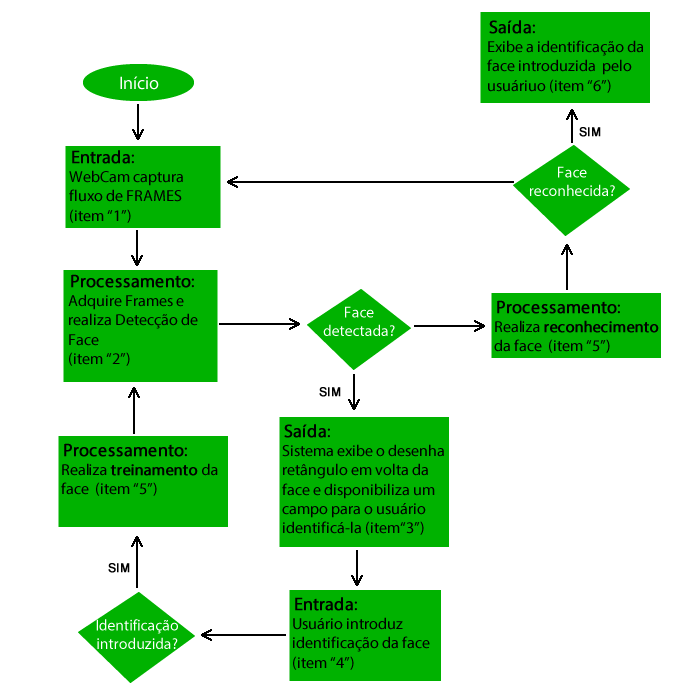
\includegraphics[width=.8\textwidth]{fluxo}
	\caption{Fluxograma representando os requisitos que devem ser atendidos.}
	\fonte{Elaborado pelo autor.}
	\label{fig:fluxoreq}
\end{figure}


\section{Diagrama de Pacotes}\label{sec:diagpacs}
Nesta seção, os pacotes criados implementação do sistema aqui proposto serão apresentadas em forma de diagrama de pacotes (UML). A \autoref{fig:SRFV_diagramaPacotes} ilustra tal diagrama:

\begin{figure}[h]
	\centering
	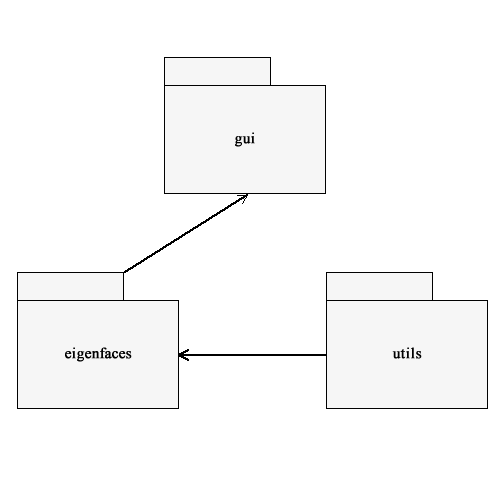
\includegraphics[width=.6\textwidth]{SRFV_diagramaPacotes}
	\caption{Diagrama de pacotes (UML) do sistema proposto.}
	\fonte{Elaborado pelo autor.}
	\label{fig:SRFV_diagramaPacotes}
\end{figure}

O pacote \textit{"gui"} possui classes responsáveis pela interface com o usuário e regras do sistema como controle de fluxo de quadros e execução de tarefas. O pacote \textit{"eigenfaces"} possui as classes responsáveis pelo execuçao do algoritmo ACP e a geração do espaço multidimensional de \textit{EigenFaces}. Por fim, o pacote de nome \textit{"utils"}, possui classes utilitárias resposáveis por manipular arquivos (carregar, salvar e deletar) e conversões de formatos de imagens. 

Na seção seguinte, cada pacote será descrito com seus respectivos diagramas de classe.

\section{Diagrama de Classes - Pacote \textit{\textbf{gui}}}\label{sec:diagclasses}
As classes do pacote \textbf{\textit{gui}} são representadas pelo diagrama (UML) na \autoref{figSRFV_diagramaClassse_gui}.

\begin{figure}[h]
	\centering
	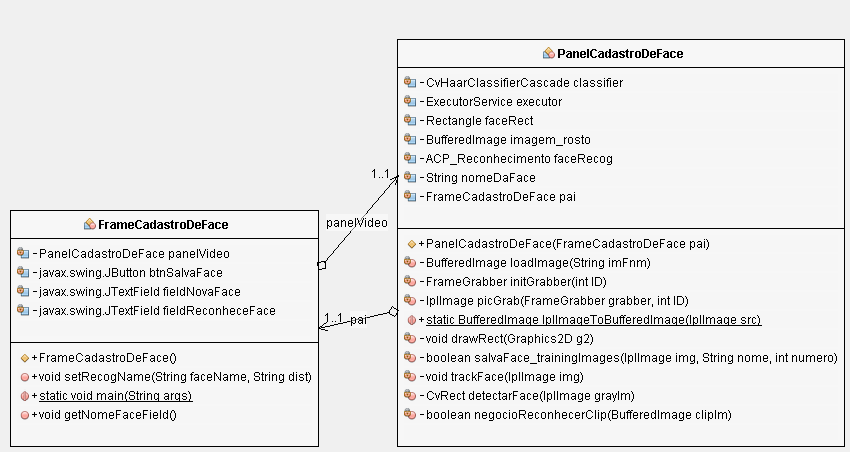
\includegraphics[width=.9\textwidth]{SRFV_diagramaClassse_gui}
	\caption{Diagrama de classes (UML) do pacote \textbf{\textit{gui}}.}
	\fonte{Elaborado pelo autor.}
	\label{figSRFV_diagramaClassse_gui}
\end{figure}

A classe \textbf{\textit{FrameCadastroDeFace}} é apenas uma janela com alguns componentes visuais, como um botão, um campo para entrada de informação e a tela para a visualizaçào do fluxo de quadros. A tela para visualização do fluxo é representada pela classe \textbf{\textit{PanelCadastroDeFace}}.

A classe \textbf{\textit{PanelCadastroDeFace}} também é responsávem pelo controle de frames e de execução de tarefas como a de deteção, treinamento e reconhecimento das faces. A seguir suas principais objetos e métodos são detalhados:

\begin{itemize}
	\item Objetos:
	\begin{itemize}
		\item \textbf{CvHaarClassifierCascade classifier}: classificadores pré treinados, assim como descritos na ????, para o processo de detecção da face;
		
		\item \textbf{ExecutorService executor:} este objeto é uma \textit{thread}. responsável por executar e controlar o processo de aquisiçao de quadros, deteção treinamento e reconecimento;
		
		\item \textbf{Rectangle faceRect:} objeto contendo a posição da face recem detectada em relação ao quadro retirado do vídeo;
		
		\item \textbf{BufferedImage imagem\_rosto:} objeto que salva um a imagem da face, caso detectada;
		
		\item \textbf{String nomeDaFace:} objeto que salva o nome da face detectada, informação esta que é entrada pelo usuário do sistema;
		
		\item \textbf{FrameCadastroDeFace pai:} objeto que referencia o seu parente de nível superior da classe \textbf{\textit{PanelCadastroDeFace}};
		
		\item \textbf{ACP\_Reconhecimento faceRecog:} objeto que instancia a classe responsável por executar o algoritmo de reconhecimento ACP, contido no pacote \textbf{\textit{eigenfaces}};
		
		\item \textbf{ACP\_Treinamento:} esta classe, contida no pacote \textbf{eigenfaces}, nao é instanciada como objeto porém é chamada de forma estática para produzir o espaço multidimensional a partir das imagens de treinamnto salvas em uma pasta especifica;
		
	\end{itemize}
	
	\item Métodos:
	\begin{itemize}
		\item \textbf{BufferedImage loadImage():} método que carrega imagem do sistema de arquivos para memória;
		
		\item \textbf{FrameGrabber initGrabber():} estabelece fluxo de quadros com a câmera;
		
		\item \textbf{IpiImage picGrab():} aquisita um quadro proveniente do fluxo de quadros;
		
		\item \textbf{void drawRect():} desenha um quadrado em volta do rosto aquisitado de acordo com as coordenadas do objeto \textbf{faceRect};
		
		\item \textbf{void salvaface\_treinamento()}: este método salva a face continda no objeto \textbf{imagem\_rosto} para futuro processo de treinamento;
		
		\item \textbf{void trackFace():} método chamado dentro da \textit{thread} ExecutorService executor que contém os processos e os controles de estado de detecção, treinamento e reconhecmento da face;
		
		\item \textbf{boolefan negocioReconhecerClip():} método chamado quando o sistema se encontra no estado de reconhecimento, onde o objeto \textbf{ACP\_Reconhecimento faceRegoc} é acionado;
	\end{itemize}
\end{itemize}

\section{Diagrama de Classes - Pacote \textit{\textbf{eigenfaces}}}\label{sec:diagclasses}
As classes do pacote \textbf{\textit{eigenfaces}} são representadas pelo diagrama (UML) da \autoref{figSRFV_diagramaClassse_eigenfaces} e descritas em seguida.

\begin{figure}[h]
	\centering
	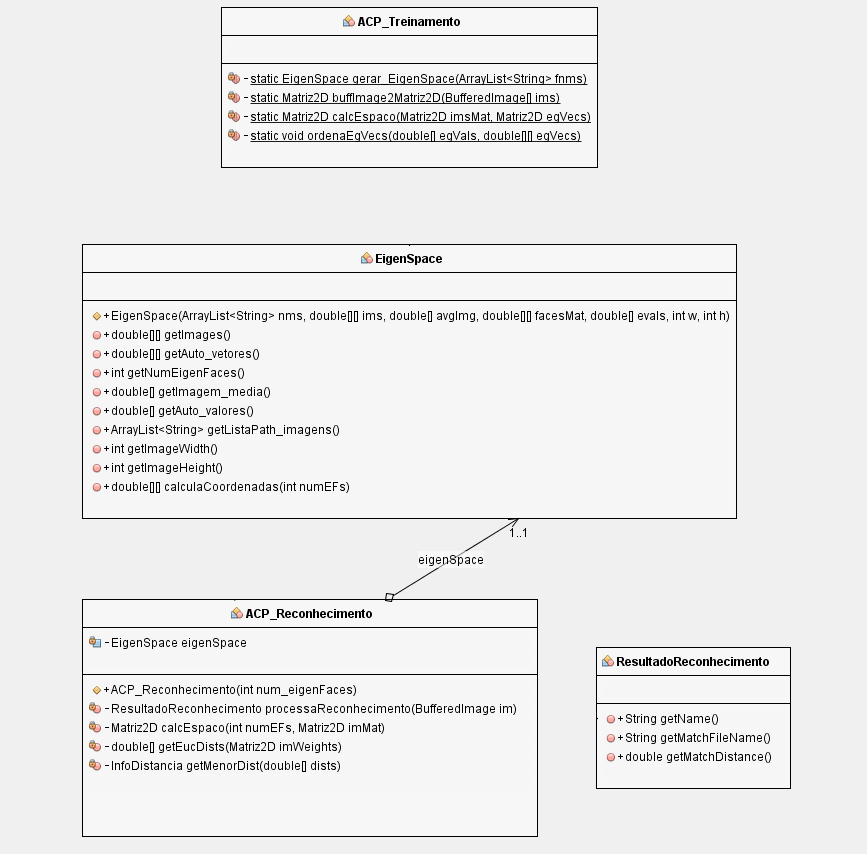
\includegraphics[width=1\textwidth]{SRFV_diagramaClassse_eigenfaces}
	\caption{Diagrama de classes (UML) do pacote \textbf{\textit{eigenfaces}}.}
	\fonte{Elaborado pelo autor.}
	\label{figSRFV_diagramaClassse_eigenfaces}
\end{figure}






\section{Diagrama de Classes - Pacote \textit{\textbf{utils}}}\label{sec:diagclasses}
As classes do pacote \textbf{\textit{utils}} são representadas pelo diagrama (UML) da \autoref{figSRFV_diagramaClassse_utils}. 

\begin{figure}[h]
	\centering
	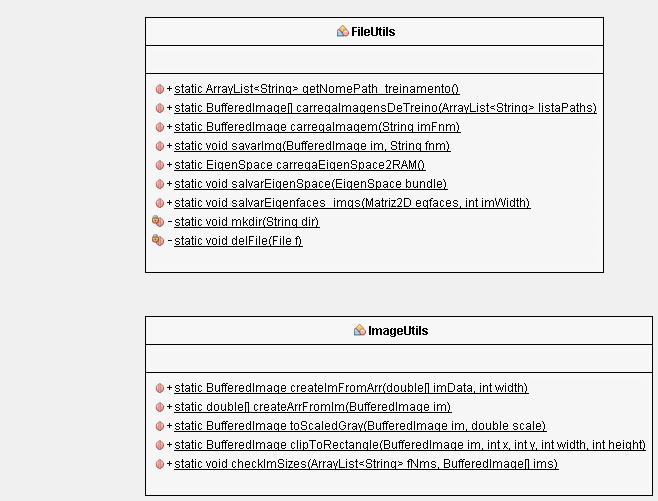
\includegraphics[width=.7\textwidth]{SRFV_diagramaClassse_utils}
	\caption{Diagrama de classes (UML) do pacote \textbf{\textit{utils}}.}
	\fonte{Elaborado pelo autor.}
	\label{figSRFV_diagramaClassse_utils}
\end{figure}












%\codigoPython
%\lstinputlisting[language=Python, label=coleta-script, caption=\textit{Script} coletar-hashtags.py]{src/coletar-hashtags.py}
